\documentclass[a4paper, 12pt]{report}
\usepackage{cmap}
\usepackage{amssymb}
\usepackage{amsmath}
\usepackage{graphicx}
\usepackage{amsthm}
\usepackage{upgreek}
\usepackage{setspace}
\usepackage[T2A]{fontenc}
\usepackage[utf8]{inputenc}
\usepackage[normalem]{ulem}
\usepackage{mathtext} % русские буквы в формулах
\usepackage[left=2cm,right=2cm, top=2cm,bottom=2cm,bindingoffset=0cm]{geometry}
\usepackage[english,russian]{babel}
\usepackage[unicode]{hyperref}
\newenvironment{Proof} % имя окружения
{\par\noindent{$\blacklozenge$}} % команды для \begin
{\hfill$\scriptstyle\boxtimes$}
\newcommand{\Rm}{\mathbb{R}}
\newcommand{\Cm}{\mathbb{C}}
\newcommand{\Z}{\mathbb{Z}}
\newcommand{\I}{\mathbb{I}}
\newcommand{\N}{\mathbb{N}}
\newcommand{\rank}{\operatorname{rank}}
\newcommand{\Ra}{\Rightarrow}
\newcommand{\ra}{\rightarrow}
\newcommand{\FI}{\Phi}
\newcommand{\Sp}{\text{Sp}}
\renewcommand{\leq}{\leqslant}
\renewcommand{\geq}{\geqslant}
\renewcommand{\alpha}{\upalpha}
\renewcommand{\beta}{\upbeta}
\renewcommand{\gamma}{\upgamma}
\renewcommand{\delta}{\updelta}
\renewcommand{\varphi}{\upvarphi}
\renewcommand{\phi}{\upvarphi}
\renewcommand{\tau}{\uptau}
\renewcommand{\lambda}{\uplambda}
\renewcommand{\psi}{\uppsi}
\renewcommand{\mu}{\upmu}
\renewcommand{\omega}{\upomega}
\renewcommand{\d}{\partial}
\renewcommand{\xi}{\upxi}
\renewcommand{\epsilon}{\upvarepsilon}
\newcommand{\intx}{\int\limits_{x_0}^x}
\newcommand\Norm[1]{\left\| #1 \right\|}
\newcommand{\sumk}{\sum\limits_{k=0}^\infty}
\newcommand{\sumi}{\sum\limits_{i=0}^\infty}
\newtheorem*{theorem}{Теорема}
\newtheorem*{cor}{Следствие}
\newtheorem*{lem}{Лемма}
\title{\textbf{\Huge{Численные методы}}\\Конспект по 3 курсу 
	специальности «прикладная математика»\\(лектор А. М. Будник)}
\date{}
\begin{document}
	\maketitle
	\tableofcontents{}
	\newpage
	\chapter{Методы решения нелинейных уравнений.}
	В данной главе будут рассмотрены некоторые методы решения нелинейных уравнений и систем уравнений. Рассмотрим случай одного нелинейного уравнения.
	\section{Постановка задачи.}
	Пусть задана функция $f(x)$ действительного переменного $x \in \Rm$. Требуется найти корни уравнения $$f(x) = 0,\eqno(1)$$
	или, что то же самое, нули функции $f(x)$. 
	Выясним, является ли задача корректно поставленной. Для ответа на вопрос существования и единственности решения введем теорему из математического анализа.
	\begin{theorem}
		Если функция $f(x)$ непрерывна на отрезке $[a,b]$ и принимает на его концах значения разных знаков, то на этом отрезке существует по крайней мере один корень уравнения $f(x) = 0$.
		Если при этом функция $f(x)$ будет монотонной на отрезке $[a,b]$, то она может иметь только один корень.
	\end{theorem}
	\begin{Proof}
		Без доказательства.
	\end{Proof}\\\\
	Выясним условие устойчивости для рассматриваемой задачи. Как правило, в качестве входных данных мы имеем функцию $f(x)$, заданную в виде функциональной формы. Поэтому понятие устойчивости здесь отпадает.
	\\\\
	Нелинейное уравнение в зависимости от вида функции $f(x)$ можно разделить на два класса:
	\begin{enumerate}
		\item алгебраические;
		\item трансцендентные.
	\end{enumerate}
	В первом классе функция $f(x)$ содержит только алгебраические функции. Например, полином $P_n(x)$ является целой алгебраической функцией. Ко второму классу относятся все другие функции, которые содержат выражения тригонометрические, показательные, логарифмические и так далее.\\\\
	Методы решения нелинейных уравнений делятся на прямые и итерационные. Мы будем рассматривать лишь итерационные методы. \\\\
	Задача нахождения корней уравнения (1) обычно решается в два этапа:
	\begin{enumerate}
		\item отделение корней;\\\\
		На этом этапе изучается расположение корней в общем случае на комплексной плоскости, проводится их разделение, т.е. выделяются области, содержащие только один корень. Кроме того изучается вопрос о кратности корней. Находятся некоторые начальные приближения $x^0$ для точного решения.
		\item построение метода.
		\\\\
		На этом этапе, используя заданное начальное приближение, строится итерационный процесс, позволяющий уточнить значение отыскиваемого корня до некоторой заданной точности $\epsilon$. Т.е., зная $x^0$, строим последовательность $x^k \xrightarrow[k\to\infty]{\epsilon}x^*$.
	\end{enumerate}
	В заключение этого параграфа запишем несколько соображений, касающихся первого этапа. По отделению корней мы можем выделить несколько способов нахождения начального приближения:
	\begin{itemize}
		\item из физических соображений;
		\item графический способ;
		\item построение таблицы значений функции $f(x)$ на заданной сетке узлов;
		\item метод деления отрезка пополам (метод дихотомии, метод бисекции).
	\end{itemize}
	Метод деления отрезка пополам заключается в том, что мы берем отрезок $[a,b]$ и смотрим, чтобы на этом отрезке функция меняла знак. Затем делим отрезок пополам, берем точку $c : a<c<b$ и в зависимости от того, где меняется знак, переходим к следующему отрезку и так далее. В итоге мы придем к тому, что отрезок получится меньше $\epsilon$, то есть мы и получим искомый корень. Число делений отрезка пополам $N \geq \log_2 \dfrac{b-a}{\epsilon}$.
	\section{Метод простой итерации решения нелинейного уравнения.}
	Применение метода требует предварительного приведения уравнения $f(x) = 0$ к каноническому виду 
	$$x = \varphi(x), \eqno(1)$$ где $\varphi(x)$ --- это заданная функция. Метод простой итерации будет иметь следующий вид: $$x^{k+1} = \varphi(x^k),\ k = 0,1,2,\ldots,\eqno(2)$$
	где $x^k$ --- последовательность, начинающаяся с $x^0$, которая должна сходится к точному решению. Область изменения аргумента $x$ на числовой оси обозначим через $X$, а через $Y$ обозначим область значений функции $y = \varphi(x)$. Тогда функцию $\varphi(x)$ можно рассматривать как оператор, преобразующий $X$ в $Y$: $$\varphi : X \to Y.$$
	Таким образом, нам нужно найти такие точки области $X$, которые при преобразовании оператором $\varphi$ переходят сами в себя, то есть точки остающиеся неподвижными при преобразовании $X$ в $Y$. Значит решения уравнения $(1)$ --- это точки, остающиеся неподвижными при преобразовании $X$ в $Y$. Геометрически это можно изобразить следующим образом: $$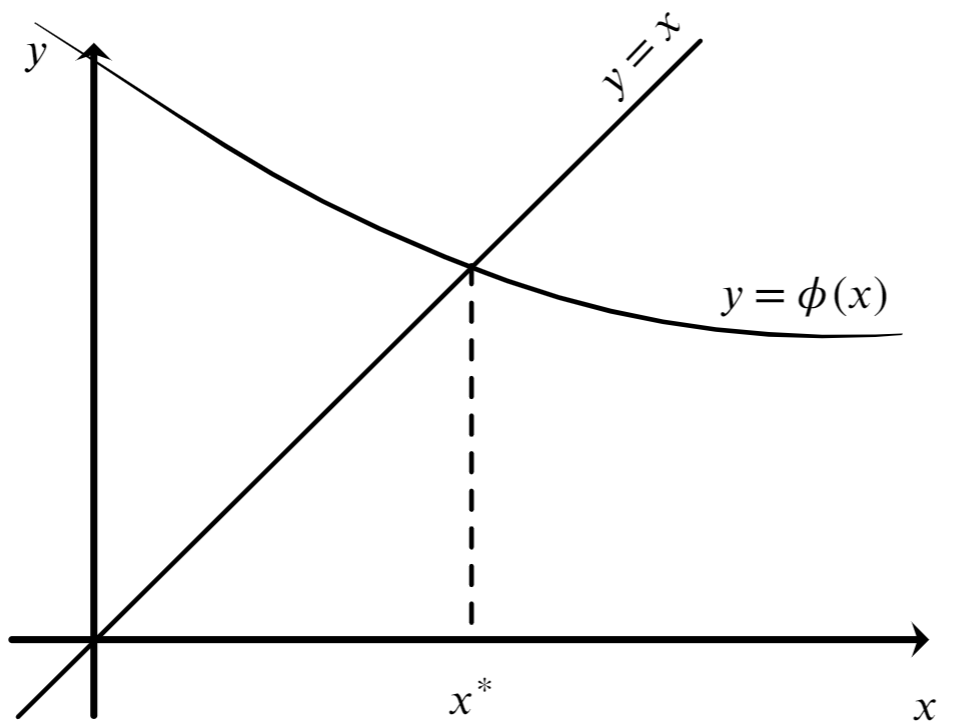
\includegraphics[scale=0.4]{img1.png}$$
	Таким образом, после процедуры отделения корней мы находим начальное приближение $x^0$ в окрестности корня $x^*$. И по найденному начальному приближению по формуле (2) строится итерационная последовательность, которая и называется \textbf{методом простой итерации.}\\\\
	Мы должны обеспечить сходимость этого итерационного процесса. Сформулируем и докажем для этого теорему.
	\begin{theorem}
		[о сходимости метода простой итерации]
		Пусть выполняются следующие условия:\begin{enumerate}
			\item функция $\varphi(x)$ определена на отрезке $$|x - x^0| \leq \delta,\eqno(3)$$ непрерывна на нем и удовлетворяет условию Липшица с постоянным коэффициентом меньше единицы, то есть $\forall x, \widetilde{x}$ $$|\varphi(x) - \varphi(\widetilde{x})| \leq q |x - \widetilde{x}| ,\quad 0 \leq q < 1;\eqno(4)$$
			\item для начального приближения $x^0$ верно неравенство $$|x^0 - \varphi(x^0)| \leq m;$$
			\item числа $\delta, q, m$ удовлетворяют условию $$\dfrac{m}{1-q}\leq \delta. \eqno(5)$$
		\end{enumerate}
		Тогда \begin{enumerate}
			\item уравнение $(1)$ в области $(3)$ имеет решение;
			\item последовательность $x^k$ построенная по правилу $(2)$ принадлежит отрезку $[x^0 - \delta, x^0 + \delta]$, является сходящейся и ее предел удовлетворяет уравнению $(1)$: $$x^k \xrightarrow[k\to \infty]{} x^*;$$
			\item скорость сходимости $x^k$ к $x^*$ оценивается неравенством $$|x^* - x^k| \leq \dfrac{m}{1- q}q^k,\ k = 1,2,\ldots \eqno(6)$$
		\end{enumerate}
		Также эта теорема может называется \textbf{методом сжимающих отображений}.
	\end{theorem}
	\begin{Proof}
		Докажем второй пункт, т.е. принадлежность.
		Методом математической индукции покажем, что при всех значениях $k=1,2,\ldots$ приближения $x^k \in [x^0 - \delta, x^0 + \delta]$ и для них верно неравенство $$|x^{k+1} - x^k| \leq mq^k.\eqno(7)$$
		При $k=0$ имеем $x^1 = \varphi(x^0)$, а $x^1$ всегда может быть найден, поскольку $\varphi$ определена в $x^0$. Кроме того $$|x^1 - x^0| = |\varphi(x^0) - x^0| \leq m,$$ т.е. формула (7) справедлива. Докажем, что $x^1$ находится не дальше, чем $m$ от $x^0$: $$m \leq \dfrac{m}{1-q}\leq \delta,$$ отсюда следует, что $x^1 \in [x^0 - \delta, x^0 + \delta]$.
		\\\\
		Пусть данное предположение справедливо при $x^0,x^1,\ldots, x^k \in [x^0 - \delta, x^0 + \delta]$ и $$|x^{n+1} - x^n| \leq mq^n,\ n = 0,1,\ldots, k-1.$$
		По предположению $x^k \in [x^0 - \delta, x^0 + \delta]$, следовательно, $x^{k+1} = \varphi(x^k)$ может быть вычислено. По сделанному допущению справедливо $$|x^k - x^{k-1}| \leq m q ^{k-1}.$$
		Теперь рассмотрим неравенство для $k+1$-ой итерации: $$|x^{k+1} - x^k| = |\varphi(x^k) - \varphi(x^{k-1})|\leq q|x^k - x^{k-1}| \leq mq^k.$$
		Осталось проверить $x^k \in  [x^0 - \delta, x^0 + \delta]$. Рассмотрим разность $$|x^{k+1} - x^0| = \Big|(x^{k+1} - x^k) + (x^k - x^{k-1}) + \ldots + (x^1 - x^0)\Big|\leq mq^k + mq^{k-1} +\ldots + m.$$
		Легко видеть, что эта сумма легко подсчитывается, как сумма геометрической прогрессии, и равна $$\dfrac{m - mq^{k+1}}{1-q} < \dfrac{m}{1-q} \leq \delta.$$
		Итак, мы доказали, что $x^{k+1}$ принадлежит отрезку (3). \\\\
		Докажем сходимость последовательности. Для этого покажем, что для последовательности выполняется условие Больцано-Коши $$|x^{k+p} - x^k| = \Big|(x^{k+p} - x^{k+p-1}) + (x^{k+p-1} - x^{k+p-2}) + \ldots + (x^{k+1} - x^k)\Big|\leq \dfrac{m}{1-q}q^k.$$
		Так как оценка не зависит от $p$ и учитывая то, что $0\leq q < 1$, можно утверждать, что признак сходимости для последовательности $x^k$ выполняется, а значит существует предел этой последовательности $$\exists \lim\limits_{k\to\infty}x^k = x^*.$$
		Нужно доказать, что $x^* \in [x^0 - \delta; x^0 + \delta]$ и $x^*$ удовлетворяет формуле (1). Это следует из того, что все $x^k$ принадлежат этому отрезку, то есть и предел находится в этом отрезке. Для доказательства второго в формуле (2) устремим $k\to\infty$: $$x^* = \varphi(x^*).$$
		Ввиду непрерывности функции, $x^*$ является решением искомого уравнения, т.е. уравнение (1) превращается в тождество.\\\\
		Последнее, что нужно доказать, --- оценка из пункта 3. Для получения неравенства (6) достаточно в соотношении $$|x^{k+p} - x^k| \leq \dfrac{m}{1-q}q^k.$$ устремить $p \to \infty$. То есть $$|x^* - x^k| \leq \dfrac{m}{1-q}q^k,$$ что и является искомой оценкой.
	\end{Proof}\\\\
	\textbf{Замечания.}\begin{enumerate}
		\item На всяком множестве точек, где для функции $\varphi(x)$ выполняется условие $$|\phi(x) - \phi(y)| <|x-y|,\ x\ne y$$ уравнение (1) может иметь не более одного решения.
		\item Пользуясь оценкой (6), можно получить априорное количество итераций, необходимое для получения приближенного решения с заданной точностью $$k \geq \dfrac{\lg \frac{\epsilon(1-q)}{m}}{\lg q}.$$
		\item Для построения сходящегося метода простой итерации в практических вычислениях условие 1 теоремы о сходимости метода простой итерации обычно заменяется более строгим требованием, а именно для всех $x$ из отрезка $|x - x^0| \leq \delta$ функция $\varphi(x)$ имеет непрерывную первую производную $\varphi'(x)$ такую, что $$|\varphi'(x)|<1 \quad \forall x \in [x_0 - \delta; x_0 + \delta].$$
		Более того, если $0\leq\varphi'(x)<1$, то поведение последовательных приближений будет монотонным. Если $-1<\varphi'(x)\leq 0$, то поведение итерационной последовательности будет колебательным.\\\\
		Геометрический смысл метода простой итерации продемонстрируем на графике:
		$$
			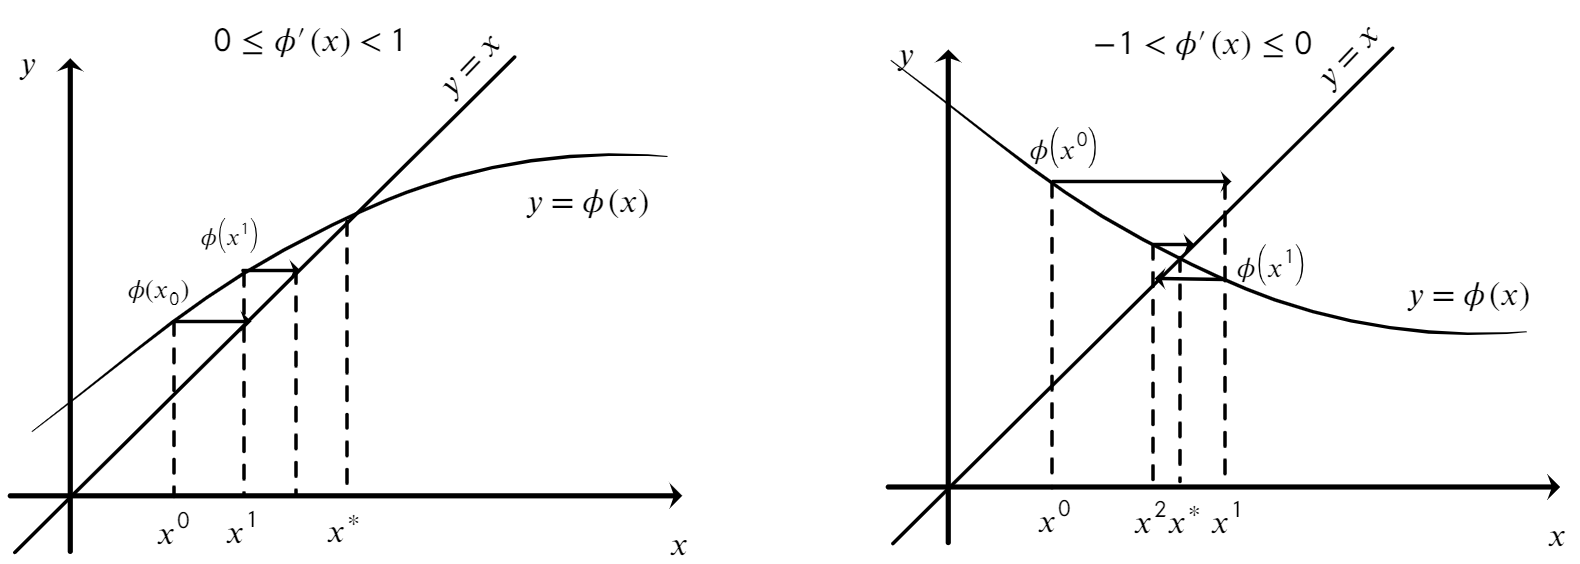
\includegraphics[scale=0.5]{img2}
		$$
		В свою очередь, при $\varphi'(x) > 1$ процесс расходится, это можно увидеть из графика 
		$$
			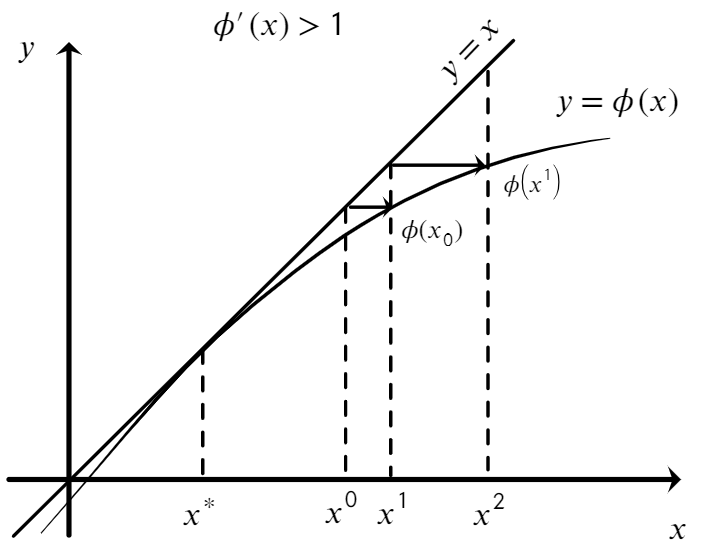
\includegraphics[scale=0.5]{img4}
		$$
		\item Так как сходимость метода простых итераций возможна при сжимающем отображении, то условие $|\varphi'(x)|<1$ является определяющим при приведении исходного уравнения к каноническому виду. \\\\
		Наиболее универсальными способом приведения к каноническому виду является преобразование $$x = \underbrace{x+f(x)}_{\varphi(x)},$$
		но нам необходимо выполнение условия $|\varphi'(x)|<1$. Поэтому мы вводим параметр $\psi(x)$, выбираемый таким образом, чтобы обеспечить сходимость: $$x = \underbrace{x+\psi(x)f(x)}_{\varphi(x)},$$ Параметр $\psi(x)$ должен быть непрерывным и  $\psi(x^*)\ne 0.$ Самый простой вариант --- взять постоянную функцию $\psi(x)=\operatorname{const}$ и подобрать эту константу из условия $|\varphi'(x)|<1$.
		\item Поведение последовательности приближений мы будем исследовать, изучая величину $$\epsilon_k = x^* - x^k$$ --- \textbf{погрешность приближенного решения на $k$-ой итерации}. Из этого соотношения легко увидеть, что $$x^k = x^* - \epsilon_k$$ и подставим это в формулу (2). Тогда $$x^* - \epsilon_{k+1} = \varphi(x^* - \epsilon_k).$$
		Предполагая, что функция $\varphi(x)$ имеет непрерывную производную в окрестности точек $x_k$ и $x_{k+1}$, разложим правую часть в ряд Тейлора в окрестности $x^*$:
		$$x^* - \epsilon_{k+1} = \varphi(x^*) - \varphi'(x^*)\epsilon_k + O(\epsilon_k^2).$$ Такое разложение возможно при условии, что функция $\varphi(x)$ дифференцируема и при предположении достаточной малости $\epsilon_k$, чтобы мы могли отбросить остальные члены. Учитывая $x^* = \varphi(x^*)$ и отбрасывая достаточно малые слагаемые $O(\epsilon_k^2)$, получим $$\epsilon_{k+1} \approx \varphi'(x^*)\epsilon_k.\eqno(8)$$
		Формула (8) дает ответ о скорости сходимости метода простой итерации. То есть погрешность на каждой итерации уменьшается по сравнению с предыдущей в величину $\varphi'(x^*)$. Таким образом, \begin{enumerate}
			\item нам нужно обеспечить $|\varphi'|<1$, чтобы $\epsilon_{k+1} < \epsilon_k$;
			\item сходимость метода осуществляется по закону геометрической прогрессии со знаменателем $q = \varphi'$.
		\end{enumerate}
	\end{enumerate}
	\section{Метод Ньютона решения нелинейного уравнения.}
	Рассмотрим уравнение $$f(x) = 0,\eqno(1)$$ где $f(x)$ достаточно гладкая функция вещественного переменного. Предположим, что для точного решения $x^*$ каким-либо образом задано начальное приближение $x^0$. Для построения метода рассмотрим погрешность $\epsilon_0 = x^* - x^0$. В предположении, что $\epsilon_0$ достаточно малая по модулю величина, подставим в уравнение (1) $x^*$ вместо $x$, тогда $$f(x^0 + \epsilon_0)=0.$$
	Разложим это выражение в ряд Тейлора в окрестности точки $x^0$:$$f(x^0 + \epsilon_0) = f(x^0) + \epsilon_0 f'(x^0) + O(\epsilon_0^2) = 0.$$
	Теперь отбросим слагаемое $O(\epsilon_0^2)$ и получим в рамках отброшенной величины получим приближенное уравнение $$f(x^0) + \epsilon_0 f'(x^0)\approx 0.$$
	Решая это уравнение относительно $\epsilon_0$, получим $$\epsilon_0 \approx -\dfrac{f(x^0)}{f'(x_0)}.$$
	Тогда выразим из $x^* = x^0 + \epsilon_0$ и учитывая, что равенство приближенное, получим $$x^* \approx x^0 - \dfrac{f(x^0)}{f'(x_0)}.$$
	В итоге, повторяя описанную процедуру, мы можем построить итерационную формулу, которая носит название \textbf{метода Ньютона} $$x^{k+1} = x^k - \dfrac{f(x^k)}{f'(x^k)},\quad k = 0,1,\ldots;\quad x_0\eqno(2)$$
	(добавка $x_0$ означает, что начальное приближение задано).
	Иногда этот метод называют \textbf{методом касательных}. Это название следует из геометрического смысла.
	Если рассмотреть уравнение кривой $y = f(x)$, то в точке $x^k$ касательная к ней задается уравнением $$y - f(x^k) = f'(x^k) (x-x^k).$$ Находим точку пересечения касательной с осью $Ox$, полагая $y=0$, и тогда $$x= x^k - \dfrac{f(x^k)}{f'(x^k)}.$$ Таким образом строим приближение $x^{k+1}$ и так далее:
	$$
		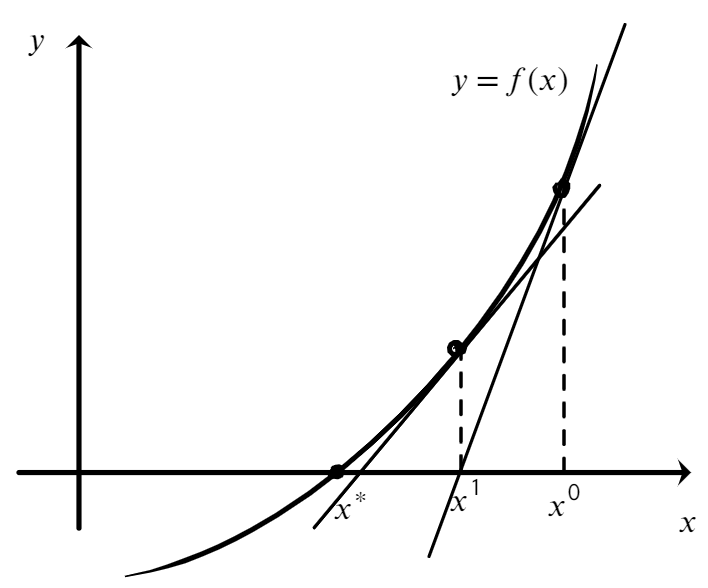
\includegraphics[scale=0.5]{img3}
	$$
	То есть мы приближаемся к корню по последовательности касательных прямых.\\\\
	Выясним, какова скорость сходимости этого метода. С помощью подстановки получим формулу для скорости сходимости $$\epsilon_{k+1} = \dfrac{\epsilon_k f'(x^* - \epsilon_k) + f(x^* - \epsilon_k)}{f'(x^* - \epsilon_k)}.$$ 
	Для того, чтобы получить ответ на вопрос, какова скорость сходимости, необходимо сделать несколько преобразований данного выражения. Воспользуемся тем, что мы можем разложить функции в ряд Тейлора в окрестности $x^*$: $$f(x^* - \epsilon_k) = f(x^*) - \epsilon_kf'(x^*) + \dfrac{1}{2}\epsilon_k^2 f''(x^*) + O(\epsilon_k^3),$$
	$$f'(x^* - \epsilon_k) = f'(x^*) - \epsilon_kf''(x^*) + \dfrac{1}{2}\epsilon_k^2 f'''(x^*) + O(\epsilon_k^3).$$
	В итоге после подстановки мы получим формулу $$\epsilon_{k+1} =- \dfrac{1}{2} \dfrac{f''(x^*)}{f'(x^*)}\epsilon_k^2 + O(\epsilon_k^3).$$
	Отбросив величину более высокого порядка, чем $\epsilon_k^2$, мы получим приближенное равенство $$\epsilon_{k+1} \approx - \dfrac{1}{2} \dfrac{f''(x^*)}{f'(x^*)}\epsilon_k^2=\alpha\epsilon_k^2. \eqno(3)$$
	Формула (3) доказывает, что при $|\alpha|<1$ последовательность $x^k$ построенная по формуле (2) обладает квадратичной сходимостью.
	\begin{theorem}
		[о сходимости метода Ньютона]
		Пусть выполняются следующие условия:
		\begin{enumerate}
			\item Функция $f(x)$ определена и дважды непрерывно дифференцируема на отрезке $$s_0 = [x^0; x^0 + 2h_0],\quad h_0 =- \dfrac{f(x^0)}{f'(x^0)}.$$
			При этом на концах отрезка $f(x)f'(x)\ne 0$.
			\item Для начального приближения $x^0$ выполняется неравенство $$2|h_0|M \leq |f'(x_0)|,\quad M = \underset{x\in s_0}{\max}|f''(x)|.$$
		\end{enumerate}
		Тогда справедливы следующие утверждения: \begin{enumerate}
			\item Внутри отрезка $s_0$ уравнение $f(x) = 0$ имеет корень $x^*$ и при этом этот корень единственный.
			\item Последовательность приближений $x^k$, $k=1,2,\ldots$ может быть построена по формуле $(2)$ с заданным приближением $x^0$.
			\item Последовательность $x^k$ сходится к корню $x^*$, то есть $x^k \xrightarrow[k\to\infty]{}x^*$.
			\item Скорость сходимости характеризуется неравенством $$|x^* - x^{k+1}|\leq |x^{k+1} - x^k|\leq \dfrac{M}{2|f'(x^*)|}\cdot (x^k-x^{k-1})^2,\quad k=0,1,2,\ldots\eqno(4)$$
		\end{enumerate}
	\end{theorem}
	\begin{Proof}
		Сначала докажем утверждение 2, т.е., что последовательность приближений $x^k$ может быть построена. Будем доказывать по индукции. По условию 1 теоремы первый член последовательности (2) можно построить $$x^1 = x^0 - \dfrac{f(x_0)}{f'(x_0)},\quad f'(x_0) \ne 0.$$
		Чтобы доказать возможность построения $x^2$, докажем, что $x^1 \in s_0$ и $f'(x^1)\ne 0$. Учитывая тот факт, что $$x_1  = x_0 + h_0,$$
		получим тот факт, что $x^1$ является серединой отрезка $s_0$. Далее рассмотрим следующее выражение, пользуясь вторым условием, теоремы $$|f'(x^1) - f'(x^0)| = \Big|\int\limits_{x^0}^{x^1} f''(x_0)dx\Big|\leq M|x^1 - x^0| = M | h_0|\leq \dfrac{|f'(x^0)|}{2}.$$
		Теперь рассмотрим $$|f'(x^1)| = \big|f'(x^0) - (f'(x^0) - f'(x^1))\big|\geq |f'(x_0)| - |f'(x^0) - f'(x^1)|\geq |f'(x^0)| - \dfrac{|f'(x^0)|}{2} = \dfrac{|f'(x_0)|}{2} \ne 0.$$
		Таким образом, $f'(x^1)\ne 0$, а значит $x^2$ может быть построено. Тогда $$x^2 = x^1 + h_1,\quad h_1 = -\dfrac{f(x^1)}{f'(x^1)}.$$
		И так далее все $x^k$ могут быть вычислены.\\\\
		 Рассмотрим, как себя ведут отрезки для того, чтобы доказать сходимость итерационного процесса. Наряду с отрезком $s_0$ рассмотрим отрезок $$s_1 = [x^1; x^1 + 2h_1].$$
		Середина этого отрезка --- это $x^2$. Покажем, что $s_1 \subset s_0$. Для этого нам нужно показать, что $h_1 < h_0$. Оценим величину $h_1$. Для этого используем разложение в ряд Тейлора: $$|f(x^1)| = \Big|f(x^0) + h_0f'(x^0) + \dfrac{h_0^2}{2}f''(x^0 + \theta h_0)\Big| = \Big|\dfrac{h_0^2}{2}f''(x^0 + \theta h_0)\Big|\leq \dfrac{h_0^2}{2}M.$$
		$$|h_1| = \Big|-\dfrac{f(x^1)}{f'(x^1)}\Big|\leq \dfrac{h_0^2}{2}\dfrac{M}{|f'(x^1)|}\leq \dfrac{h_0^2}{2}\dfrac{2M}{|f'(x^0)|} = h_0\dfrac{M}{|f'(x^0)|}\leq \dfrac{|h_0|}{2}.$$
		Итак $2|h_1| \leq |h_0|$, следовательно, $$x^1 + 2h_1 = x^0 + h_0 + 2h_1 \leq x^0 + 2h_0 \in s_0.$$
		Отсюда следует, что $s_1 \subset s_0$.\\\\
		Далее мы можем показать по индуктивному предположению, что на отрезке $s_1$ итерация $x^1$ будет удовлетворять условиям 1 и 2 теоремы. Обе части неравенства $|h_1|\leq \dfrac{|h_0|}{2}$ домножим на $\dfrac{2M}{|f'(x^1)|}$, тогда $$\dfrac{2M}{|f'(x^1)|}|h_1|\leq \dfrac{2|h_0| M}{2|f'(x^1)|}$$
		Воспользуемся ранее произведенными оценками:
		$$2|h_0| M \leq |f'(x^0)|,\quad 2|f'(x^1)|\geq \dfrac{1}{2}|f'(x^0)|$$
		Тогда $$\dfrac{2|h_0| M}{2|f'(x^1)|} \leq 1\Rightarrow 2|h_1| M \leq |f'(x^1)|.$$
		Таким образом, на отрезке $s_1$ функция $f(x)$ удовлетворяет условиям теоремы 1 и 2. Теперь по индукции очевидна возможность построения последовательности $x^{k+1}$ по формуле (2). При этом $x^{k+1}$ является серединой отрезка $$s_k = [x^k; x^k + 2h_k], \quad h_k = -\dfrac{f(x^k)}{f'(x^k)}.$$
		А отрезок $s_k\subset s_{k-1}$ и не превосходит половины длины $s_{k-1}$. Кроме того, выполняется неравенство, являющегося оценкой половины длины отрезка $$|h_k| \leq \dfrac{h_{k-1}^2M}{2|f'(x^k)|}.$$
		То есть мы доказали утверждение 2.\\\\
		Докажем утверждения 3 и 1. Так как мы построили последовательность вложенных отрезков $$s_k \subset s_{k-1}\subset \ldots \subset s_1 \subset s_0,$$ длины которых с ростом $k$ стремятся к нулю, то, таким образом, эти отрезки стягиваются в точку. А следовательно последовательность $x^{k+1}$, элементы которой являются серединами этих отрезков, также является сходящейся к некоторому значению $x^*$. Отсюда $$x^{k+1}\xrightarrow[k\to\infty]{} x^*,$$
		но существование предела еще не означает, что это нужный нам предел. Покажем, что $x^*$ -- это корень уравнения (1). Для этого в формуле (2) перейдем к пределу при $k\to\infty$: $$x^* = x^* - \dfrac{f(x^*)}{f'(x^*)},$$ но дробь нужно рассмотреть отдельно. Для того, чтобы перейти к пределу в $f(x^k)$, мы должны доказать, что $$\lim\limits_{k\to\infty}f(x^k) = f(\lim\limits_{k\to\infty}x^k),$$
		этот переход возможен в силу непрерывности функции $f$ и в силу того, что $f'(x^k)\ne 0$ $\forall k$. Тогда записанная нами формула будет верна. А из этой формулы можно сделать вывод, что $$f(x^*) =0.$$
		Теперь докажем единственность этого корня $x^*$. Для этого предположим, что $M > 0$ (случай $M = 0$ мы не рассматриваем, иначе функция будет линейной, а в таком случае на первой же итерации мы получим точное решение). По условию теоремы $$f'(x^0) \ne 0,\quad f'(x^0 + 2h_0) \ne 0.$$
		Учитывая этот факт, мы можем утверждать, что $$f'(x) \ne 0,\quad \forall x \in s_0,$$
		действительно докажем это. Для этого рассмотрим любую точку отрезка $x \in s_0$: $$|f'(x) - f'(x^0)|  = \Big|\int\limits_{x^0}^x f''(t)dt\Big|\leq M|x-x^0| < M \cdot 2|h_0|\leq |f'(x^0)|.$$
		Теперь мы можем оценить величину $\forall x \in s_0$ $$|f'(x)| = |f'(x^0) - (f'(x^0) - f'(x))| \geq |f'(x^0)| - |f'(x^0) - f'(x)|>  |f'(x^0)| - |f'(x_0)| = 0.$$
		То есть $f'(x)\ne 0$ в любой точке отрезка $s_0$. Этот факт говорит о том, что $f(x)$ строго монотонна на $s_0$. Следовательно, уравнение (1) имеет не более одного корня.\\\\
		Докажем утверждение 4. По доказанным ранее утверждениям $x^{k+1}$ --- это середина отрезка $s_k$ длиной $2|h_k|$ и $x^* \in s_k$. Тогда можно рассмотреть $$|x^* - x^{k+1}| \leq |h_k|\leq \dfrac{h_{k-1}^k M}{2 |f'(x^1)|},\ k=0,1,\ldots$$
		Отсюда и следует формула (4).
	\end{Proof}\\\\
	\textbf{Замечания.}\begin{enumerate}
		\item Из оценки (4) можно получить априорную оценку количества итераций, необходимых для достижения заданной точности $\epsilon$ (доказать самостоятельно)
		$$ k \geq \log_2 \dfrac{\ln(\alpha \epsilon)}{\ln(\alpha |x^1 - x^0|)},\quad \alpha = \underset{x\in s_0}{\max}\Big|\dfrac{f''(x)}{2f'(x)}\Big|.$$
		\item Если в окрестности корня производная $f'(x)$ сохраняет знак и монотонна, то приближение $x_k$ построенное по формуле (2) сходится с одной стороны.
	\end{enumerate}
	\section{Видоизменения метода Ньютона и метода простой итерации.}
	\subsection{Модификации метода Ньютона.}
	Все видоизменения связаны с тем, что мы хотим упростить формулу метода Ньютона и уменьшить количество арифметических операций, а для этого будем пытаться заменить вычисление производной вычислением другой более простой функции.
	\subsubsection{Метод Ньютона с постоянной производной.}
	Формула этого метода имеет следующий вид $$x^{k+1} = x^k - \dfrac{f(x^k)}{f'(x^0)},\ k=0,1,\ldots,\quad x^0.$$
	Это видоизменение напрямую связано с уменьшением количества арифметических операции, поскольку мы отказываемся от вычисления последовательности $f'(x^k)$. Таким образом, с точки зрения количества операций метод простой итерации и метод Ньютона становятся сравнимы между собой.\\\\ Геометрически это означает, что, выбрав $x^0$, мы движемся по касательной. Найдя $x^1$, мы будем двигаться из точки $x^1$ по той же касательной, т.е. все касательные будут параллельны касательной в точке, которая является начальным приближением к корню.
	$$
		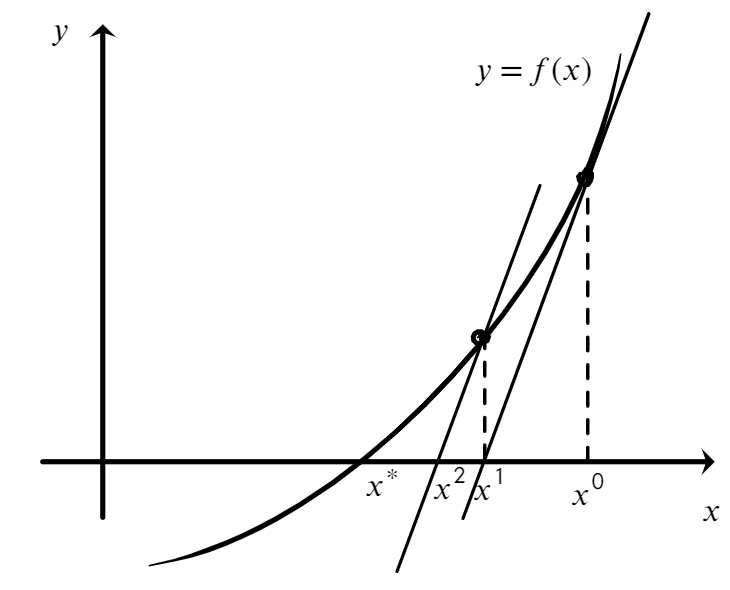
\includegraphics[scale=0.5]{img5}
	$$
	Но скорость сходимости данного метода ухудшится. Легко видеть, что погрешность на каждой итерации будет меняться по следующему закону $$\epsilon_{k+1} = \epsilon_k - \dfrac{f(x^* - \epsilon_k)}{f'(x^0)}.$$
	Проделав необходимые вычисления, связанные с разложением функции в окрестности $x^*$, можно получить $$\epsilon_{k+1}\approx\Big(1 - \dfrac{f'(x^*)}{f'(x^0)}\Big)\epsilon_k.\eqno(2)$$
	Исходя из вида формулы (2), мы можем утверждать, что такая модификация имеет линейную скорость сходимости.
	\subsubsection{Метод секущих.}
	Возьмем за основу формулу производной $$f'(x^k)\approx \dfrac{f(x^k) -f(x^{k-1})}{x^{k} - x^{k-1}},\ k = 1,2,\ldots.$$
	И, подставляя в формулу Ньютона, мы получим следующую формулу $$x^{k+1} = x^k - f(x^k)\dfrac{x^k - x^{k-1}}{f(x^k) - f(x^{k-1})},\ k = 1,2,\ldots;\ x^0\eqno(3)$$
	Однако мы должны знать не только $x^0$, но и $x^1$, поэтому метод секущих двухшаговый.\\\\
	Геометрически мы выбираем два приближения $x^0$ и $x^1$ и через две эти точки мы проводим прямую, и она является не касательной, а секущей. Таким образом, при пересечении секущей с осью $Ox$ мы получаем точку $x^2$. Проводим через $x^1$ и $x^2$ следующую секущую, получаем точку $x^3$ и так далее.
	$$
		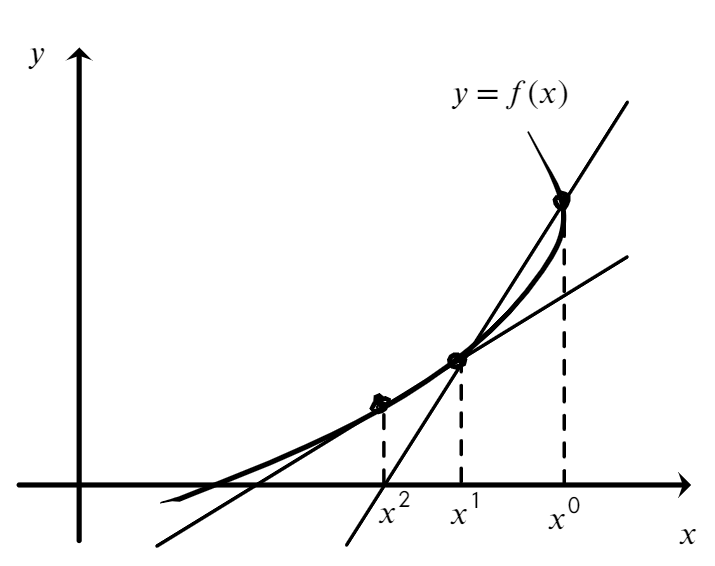
\includegraphics[scale=0.5]{img6}
	$$
Количество операций в этом случае сравнимо с количеством операций метода Ньютона с постоянной производной. Но при этом мы выигрываем в скорости, покажем это. Мы имеем следующее уравнение для погрешности:
$$\epsilon_{k+1} = \epsilon_k - \dfrac{(\epsilon_k - \epsilon_{k+1})f(x^* - \epsilon_k)}{f(x^* - \epsilon_k) - f(x^* - \epsilon_{k-1})}.$$
После выделения главной части из формулы и приведения подобных слагаемых, мы получим соотношение между погрешностями $$\epsilon_{k+1}\approx -\dfrac{1}{2} \dfrac{f''(x^*)}{f'(x^*)}\epsilon_k\epsilon_{k-1}\eqno(4)$$
Таким образом, она выше чем линейная, но ниже, чем квадратичная. Для уточнения необходимо преобразовать данную величину. Соотношение на $k+1$ и $k$ итерациях может быть оценено как $$\epsilon_{k+1}\approx C\epsilon_k^\alpha,\quad \alpha = \dfrac{1+\sqrt5}{2}.$$
\subsubsection{Метод хорд.}
Формула метода хорд имеет вид $$x^{k+1} = x^k - f(x^k)\dfrac{x^k - x^0}{f(x^k) - f(x^0)},\ k=1,2,\ldots;\ x^0, x^1\eqno(5)$$
Для подсчетов нам нужно два приближения, но сам метод одношаговый.\\\\
Геометрически мы строим хорды, проходящие через точку $f(x^0)$ и $f(x^k)$ на каждой итерации. Точка пересечения этой хорды с осью $Ox$ приводит нас к новому приближению $x^{k+1}$:
$$
	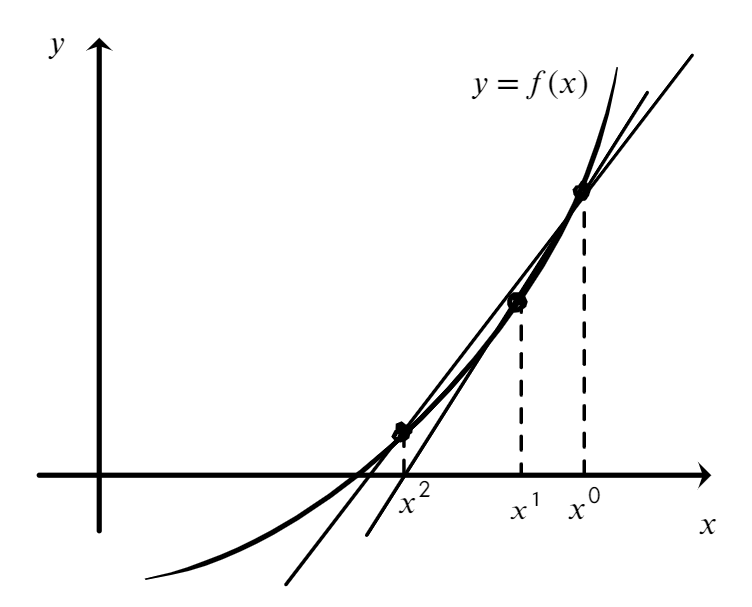
\includegraphics[scale=0.5]{img7}
$$
 В количестве операций мы не выигрываем. Можно показать, что погрешность в данном случае будет иметь вид $$\epsilon_{k+1} \approx -\dfrac{1}{2}\dfrac{f''(x^*)}{f'(x^*)}\epsilon_0\epsilon_k\eqno(6)$$
Отсюда можно сделать вывод, что метод хорд сходится по закону геометрической прогрессии, а значит по линейному закону, но знаменатель прогрессии будет зависеть от $\epsilon_0$. При достаточно хорошем начальном приближении этот метод может сходиться быстрее, чем остальные методы. Практически обычно метод хорд используется для того, чтобы сузить область, где находится корень.
\subsection{Модификации метода простой итерации.}
Все модификации сводятся к тому, что мы хотим повысить скорость сходимости метода.
\subsubsection{Метод Стеффенсена.}
Метод Стеффенсена основывается на том, что мы укажем способ вычисления $x^{k+1}$ через $x^k$ таким образом, чтобы обеспечить квадратичную скорость сходимости. Для увеличения скорости сходимости в данном методе используется преобразование Эйткена. Суть его состоит в том, что, если имеется сходящаяся последовательность чисел $s_0, s_1,\ldots, s_n,\ldots$, которая сходится к числу $s$, и при этом мы знаем, что характер сходимости носит вид $$s_n = s + Aq^n,\quad A = \operatorname{const}, q < 1,$$ то есть сходимость по закону геометрической прогрессии со знаменателем $q$. Тогда закон Эйткена позволяет сразу получить значение искомого предела по формуле Эйткена, построив последовательность $$\sigma_0,\sigma_1,\ldots,\sigma_n, \quad \sigma_n = s = \dfrac{s_{n+1}s_{n-1} - s_n^2}{s_{n+1} - 2s_n + s_{n-1}} = \lim\limits_{n\to\infty} s_n.\eqno(7)$$
Мы будем использовать эту формулу для того, чтобы сразу найти нужный нам предел в методе простой итерации. \\\\
Пусть мы имеем $x^0$. Берем приближения $$x^1 = \varphi(x^0), \quad x^2 = \varphi(x^1) = \varphi(\varphi(x^0)).$$
Тогда, используя формулу (7), мы можем при $n=1$ получить $$\sigma_1 = \dfrac{x^0x^2 - (x^1)^2}{x^2 - 2x^1 +x^0} = \dfrac{x^0 \varphi(\varphi(x^0)) - (\varphi(x^0))^2}{\varphi(\varphi(x^0)) - 2 \varphi(x^0) + x^0}.$$
Заменим в этой формуле соответствующим образом индексы. В итоге получается итерационная формула, которая получила название \textbf{метод Стеффенсена}
$$x^{k+1} = \dfrac{x^k \varphi(\varphi(x^k)) - (\varphi(x^k))^2}{\varphi(\varphi(x^k)) - 2 \varphi(x^k) + x^k},\ k=0,1,\ldots;\ x^0.\eqno(8)$$
Метод Стеффенсена можно трактовать как метод простой итерации примененный к уравнению вида $$x = \Phi(x),$$ где $$\Phi(x) = \dfrac{x \varphi(\varphi(x)) - \varphi^2(x)}{\varphi(\varphi(x)) - 2\varphi(x) + x}.$$ 
Возникает вопрос сходимости метода.
Можно доказать, что функция $\Phi(x)$ вместе со своей производной будет непрерывна в окрестности точки $x^*$, причем $$\lim\limits_{x\to x^*}\Phi(x) = x^*.$$ Если предположить, что функция $\Phi(x^*) = x^*$ (то есть мы доопределяем ее), то $\Phi(x)$ будет непрерывна в точке $x^*$. Кроме того можно утверждать, что $$\Phi'(x^*) = \lim\limits_{x\to x^*}\dfrac{\Phi(x) - \Phi(x^*)}{x - x^*} = 0.$$
Таким образом, можно утверждать, что сходимость метода Стеффенсена будет квадратичной. То есть мы построили метод, обладающий повышенной скоростью сходимости. Но в 2 раза увеличивается объем вычислений, из-за того, что нужно вычислять функцию $\varphi(\varphi(x))$.
\subsubsection{Метод Чебышева.}
Идея метода базируется на способе построения итерационного процесса таким образом, чтобы обеспечить обращение в ноль производных от функции $\varphi(x)$ в точке $x^*$, то есть мы берем уравнение $$x = \varphi(x)$$ и стараемся построить метод, у которого максимальное количество производных обращается в ноль в точке $x^*$. Для этого функцию $\varphi(x)$ запишем в виде $$\varphi(x) = x+ \psi_1(x) f(x) + \psi_2(x)f^2(x) + \ldots + \psi_{n-1}(x)f^{n-1}(x),\eqno(9)$$
где $f(x)$ --- это исходная функция, для которой мы ищем корни. Требуется выбрать функции $\psi_1(x),\ldots, \psi_{n-1}(x)$ так, чтобы $$\varphi^{(j)}(x)\Big|_{f(x)=0} = 0,\quad j=1,2,\ldots,n-1 \eqno(10)$$
Рассмотрим условие на первую производную \begin{multline*}
	\varphi'(x)\Big|_{f(x) = 0} = 1 + \psi_1'(x)f(x) + \psi_1(x) f'(x) + \psi_2'(x) f^2(x) + 2\psi_2(x) f(x) f'(x) + \ldots \Big|_{f(x) = 0}=\\=1 + \psi_1(x) f'(x) \Big|_{f(x) = 0} = 0.
\end{multline*}
Аналогичным образом мы можем записать вторую производную
$$\varphi''(x)\Big|_{f(x) = 0} = 2\psi_1' f'(x) + \psi_1(x) f''(x) + 2\psi_2(x) (f'(x))^2 \Big|_{f(x) = 0} = 0.$$
Из условия $\varphi'(x)\Big|_{f(x) = 0}=0$ следует, что функция $$\psi_1(x) = -\dfrac{1}{f'(x)}.$$ Отсюда $$\varphi(x) = x + \Big(-\dfrac{1}{f'(x)}\Big)f(x),$$ то есть мы пришли к методу Ньютона, итерационному процессу второго порядка.
Из условия, что $\varphi''(x)\Big|_{f(x) = 0}=0$, применяя простые арифметические действия, мы можем получить $$\psi_2(x) = -\dfrac{f''(x)}{2(f'(x))^3}.$$ Учитывая выражения для $\psi_1$ и $\psi_2$ мы модем построить итерационный процесс третьего порядка с кубической скоростью сходимости $$x^{k+1} = x^k - \dfrac{f(x^k)}{f'(x^k)} - \dfrac{f^2(x^k)f''(x^k)}{2(f'(x^k))^3}\eqno(11)$$ и будем называть эту формулу \textbf{методом Чебышева}. В этом методе мы также увеличиваем количество операций, так как необходимо вычислять значения $f(x), f'(x), f''(x)$.
\section{Метод Лобачевского.}
Метод Лобачевского является методом отыскания корней алгебраического уравнения. Данные метод не требует предварительного задания начального приближения для корней и кроме того позволяет найти сразу все корни.\\\\
Рассмотрим алгебраическое уравнение следующего вида $$P(x) = a_0x^n + a_1x^{n-1} + \ldots + a_{n-1}x + a_n = 0,\quad a_0 \ne 0.\eqno(1)$$
Пусть $a_i\in \Rm$ и предположим, что все корни $x_i$ простые, вещественные и удовлетворяют соотношению $$|x_1| >> |x_2| >> \ldots >> |x_n|,\eqno(2)$$ то есть отношение эквивалентно $$\dfrac{|x_{k+1}|}{|x_k|}<<1,\ k=\overline{1,n-1}.$$
Если выполняется условие (2), то говорят, что \textbf{корни сильно разделены} в смысле отношения $(k+1)$-го корня к $k$-ому. \\\\
Из алгебры известно, что соотношение Виета, связывающее корни многочлена с его коэффициентами, является системой вида $$\begin{cases}
	x_1 + x_2 + \ldots + x_n = -\dfrac{a_1}{a_0},\\
	x_1x_2 + x_1x_3 + \ldots + x_{n-1}x_n = \dfrac{a_2}{a_0},\\
	x_1x_2x_3 + \ldots + x_{n-2} x_{n-1}x_n = -\dfrac{a_3}{a_0},\\
	\dotfill\\
	x_1x_2\ldots x_n=(-1)^n\dfrac{a_n}{a_0}.
\end{cases}\eqno(3)$$
В случае выполнения соотношения (2) в левых частях соотношений (3) главными членами будут все первые слагаемые. Тогда вместо точных равенств можно записать приближенные: $$\begin{cases}
x_1 \approx -\dfrac{a_1}{a_0},\\
x_1x_2 \approx \dfrac{a_2}{a_0},\\
x_1x_2x_3 \approx - \dfrac{a_3}{a_0},\\
\dotfill\\
x_1x_2\ldots x_n \approx (-1)^n\dfrac{a_n}{a_0}.
\end{cases}$$
Отсюда можно найти приближенные значения корней
$$x_i \approx -\dfrac{a_i}{a_{i-1}}, i=\overline{1,n}.\eqno(4)$$
Если требование сильной разделенности корней не выполняется, то мы будем строить новое уравнение, корни которого будут высокими степенями корней исходного уравнения. При этом можно надеяться получить уравнение с сильно разделенными корнями. Метод Лобачевского основан на построении уравнения, корни которого являются квадратами корней исходного.\\\\
Запишем уравнение $P(x) =0$ в виде $$P(x) = a_0(x-x_1)(x-x_2)\ldots(x-x_n) =0.$$
Также рассмотрим полином $$P^*(x) = a_0(x+x_1)(x+x_2)\ldots (x+x_n)=0.$$
Корни полинома $P^*(x)$ отличаются от корней исходного уравнения только знаком. По многочленам $P(x)$ и $P^*(x)$ построим многочлен $P_1(y)$ такой, что корнями этого полинома будут являться значения $y_i = x_i^2$, $i=\overline{1,n}.$ Для этого перемножим $$P(x)P^*(x) = a_0^2(x^2 - x_1^2)(x^2 - x_2^2)\ldots(x^2 - x_n^2).$$
Сделав замену $y_i = x_i^2$, мы получим полином $P_1(y)$. Обозначим коэффициенты полинома $P_1(y)$ через $a_i^{(1)}$ и формально перемножим $P(x)$ с $P^*(x)$:
$$P(x)P^*(x) = (a_0x^n + a_{1}x^{n-1} + \ldots + a_n)(a_0x^n - a_1x^{n-1} +\ldots + (-1)^na_n).$$
Тогда коэффициенты нового полинома $$\begin{cases}
	a_0^{(1)} = a_0^2,\\
	a_1^{(1)} =2a_0a_2 - a_1^2,\\
	a_2^{(1)} = 2a_0a_4 - 2a_1a_3 + a_2^2,\\
	\dotfill\\
	a_n^{(1)} = (-1)^na_n^2.
\end{cases}\eqno(5)$$
Предположим, что на основании соотношения (5) мы можем построить последовательность многочленов $$P_k(x) = a_0^{(k)}x^n + a_1^{(k)}x^{n-1} + \ldots + a_n^{(k)}$$ и корнями каждого уравнения $P_k(x) = 0$ будут являться $x_i^{2^k}$, где $x_i$ --- корни исходного уравнения (1). Тогда на каком-то $k$-ом шаге, предполагая сильную разделенность корней, воспользуемся формулой (4) $$x_i^{2^k}\approx - \dfrac{a_i^{(k)}}{a_{i-1}^{(k)}},\quad i =\overline{1,n},$$
а отсюда мы можем извлечь корень степени $2^k$ и найти модули корней исходного уравнения, а их знаки определим подстановкой в многочлен.\\\\
Исследуем вопрос о том, сколько шагов описанного процесса (квадрирования) нужно провести, чтобы получить сильную разреженность корней. Мы укажем один из способов получения условий, который гарантирует сильную разделенность. Пусть процесс квадрирования проведен $k$ раз и мы построили полином $P_k(x)$ такой, что его корни достаточно разделены. Тогда $$\begin{cases}
x_1^{2^k}\approx -\dfrac{a_1^{(k)}}{a_0^{(k)}},\\
x_1^{2^k}x_2^{2^k}\approx \dfrac{a_2^{(k)}}{a_0^{(k)}},\\
\dotfill\\
x_1^{2^k}\ldots x_n^{2^k}\approx (-1)^n\dfrac{a_n^{(k)}}{a_0^{(k)}}.
\end{cases}$$
Теперь мы можем сделать еще один шаг квадрирования 
$$\begin{cases}
	x_1^{2^{k+1}}\approx -\dfrac{a_1^{(k+1)}}{a_0^{(k+1)}},\\
	x_1^{2^{k+1}}x_2^{2^{k+1}}\approx \dfrac{a_2^{(k+1)}}{a_0^{(k+1)}},\\
	\dotfill\\
	x_1^{2^{k+1}}\ldots x_n^{2^{k+1}}\approx (-1)^n\dfrac{a_n^{(k+1)}}{a_0^{(k+1)}}.
\end{cases}$$
Из этих двух систем видно, что $$(x_1^{2^{k+1}}) = (x_1^{2^k})^2.$$
Подставим и получим $$-\dfrac{a_1^{(k+1)}}{a_0^{(k+1)}}\approx \Big(-\dfrac{a_1^{(k)}}{a_0^{(k)}}\Big)^2 \Rightarrow a_1^{(k+1)}\approx -(a_1^{(k)})^2$$
И так далее. При достаточно больших $k$ с требуемой точностью эти величины будут равны. Значит мы достигли требуемой степени разреженности корней. Таким образом, условием того, что достигнута требуемая разделенность корней является следующая связь между коэффициентами многочлена
$$a_i^{(k+1)}\approx (-1)^i(a_i^{(k)})^2.\eqno(6)$$
Тогда, если это выполнено, $x_i$ могут быть посчитаны по формулам $$|x_i| = \sqrt[2^{k+1}]{-\dfrac{a_i^{(k+1)}}{a_{i-1}^{(k+1)}}}\eqno(7)$$
Таким образом, алгоритм метода Лобачевского определен.
\section{Методы решения систем нелинейных уравнений (СНУ).}
В общем виде СНУ можно записать как в координатном виде $$f_i(x_1,\ldots, x_n) = 0,\quad i=\overline{1,n},\eqno(1)$$ так и в векторном виде $$f(x) = 0,\quad f=(f_1,\ldots, f_n)^T,\ x = (x_1,\ldots, x_n)\eqno(1)$$
Частные случаи при $n=1$ -- одно нелинейное уравнение. Если $n>1$, но функции $f_i$ линейные, то получим СЛАУ. Поэтому рассмотрим случай, когда функции нелинейные и $n\geq 2$. Основные этапы решения СНУ:
\begin{enumerate}
	\item отделение корня;
	\item построение последовательности приближений;
	\item контроль сходимости.
\end{enumerate}
Следует иметь ввиду, что проблема отделения корня в общем случае не имеет решений.
\subsection{Метод простой итерации (МПИ).}
Применение метода простой итерации требует приведения исходной системы (1) к виду удобному для итераций, т.е. канонической форме, $$\begin{cases}
	x_1 = \varphi_1(x_1, \ldots, x_n),\\
	\dotfill,\\
	x_n = \varphi_n(x_1,\ldots, x_n);
\end{cases}\eqno(2)$$
или в векторной форме $$x = \varphi(x),\quad \varphi = (\varphi_1,\ldots, \varphi_n)^T,\ x=(x_1, \ldots, x_n).$$
Мы будем предполагать, что $x^*=(x_1^*,\ldots, x_n^*)$ --- точное решение, а $x^k = (x_1^k,\ldots, x_n^k)$ --- итерационное приближение. Если выбрано начальное приближение $x_0$, то все последующие приближения находятся по формуле $$x_{i}^{k+1} = \varphi_i(x_1^k,\ldots, x_n^k), \quad i = \overline{1,n},\ k=0,1,\ldots$$ или в векторной форме $$x^{k+1} = \varphi(x^k)\eqno(3)$$
Будем считать функции $\varphi_i(x)$ непрерывно дифференцируемыми в общей области их задания. Будем далее предполагать, что решение $x^*$ так же, как и все приближения $x^k$, лежат внутри этой области.\\\\
Выясним поведение вектора погрешности $\epsilon^k = (\epsilon_1^k,\ldots, \epsilon_n^k)$ $$\epsilon^k = x^* - x^k = (x_1^* - x_1^k,\ldots, x_n^* - x_n^k)$$
Посмотрим, как будет вести себя погрешность с увеличением количества итераций. Для этого подставим в формулу (3) выражение $x^k$ через $\epsilon^k$ и получим следующее выражение $$x_i^* - \epsilon_i^{k+1} = \varphi_i(x_1^* - \epsilon_1^k,\ldots, x_n^* - \epsilon_n^k).$$
Разложим правую часть последних равенств по степеням $\epsilon^k$ в окрестности точки $x^*$ и выделим главную часть, учитывая, что $x^* = \varphi(x^*)$. Тогда получим $$\epsilon_i^{k+1} = \sum_{j=1}^{n}\dfrac{\partial}{\partial x_j}\varphi_i(x_1^*,\ldots, x_n^*)\epsilon_j^* + O\Big(\max_j (\epsilon_j^k)^2\Big),\quad i = \overline{1,n}.$$
Если мы предположим, что $\epsilon_j^k$ достаточно малые, то можем отбросить достаточно малые слагаемые и записать приближенно отношения между $k$-ой и $(k+1)$-ой итерациями: $$\epsilon^{k+1}\approx A\epsilon^k\eqno(4)$$
где $A$ -- это матрица Якоби построенная по системе функций $\varphi_i$:
$$A = \begin{pmatrix}
	\dfrac{\partial \varphi_1(x^*)}{\partial x_1} & \dots & \dfrac{\partial \varphi_1(x^*)}{\partial x_n}\\
	\vdots & \ddots & \vdots\\
	\dfrac{\partial \varphi_n(x^*)}{\partial x_1} & \dots & \dfrac{\partial \varphi_n(x^*)}{\partial x_n}
\end{pmatrix}$$ 
Таким образом, видно что вектор погрешности на одном шаге испытывает линейное преобразование. Для того, чтобы сделать вывод об условиях сходимости, преобразуем формулу (4). Запишем спектральное разложение матрицы $A$. Предположим, что все элементарные делители матрицы $A$ являются простыми. Тогда эту матрицу можно записать в виде спектрального разложения $$A = S^{-1}\Lambda S,\quad \Lambda = \operatorname{diag}\{\lambda_1,\ldots, \lambda_n\}$$
Тогда соотношение (4) можно записать в виде $$\epsilon^{k+1} \approx S^{-1}\Lambda S \epsilon^k.$$
Обозначим $$r^k = S \epsilon^k.$$
Домножим обе части слева на $S$, тогда $$r^{k+1}\approx \Lambda r^k$$
или покоординатно $$r_i^{k+1} = \lambda_i r^k_i,\quad i=\overline{1,n}$$
Если все $|\lambda_i| <1$ $\forall i$, то $$r_i^k\xrightarrow[k\to \infty]{}0.$$ По условию $\epsilon^k = S^{-1}r^{k}$, а значит $$\epsilon^k\xrightarrow[k\to \infty]{}0.$$
Тогда можно утверждать, что $$x^k\xrightarrow[k\to\infty]{} x^*.$$
Таким образом, необходимым и достаточным условием сходимости является условие $|\lambda_i| <1$ $\forall i$ (по аналогии с МПИ для СЛАУ). Но в практических целях проверка этого условия достаточно затруднительна. Сформулируем теорему о достаточных условиях сходимости МПИ в случае СНУ.
\begin{theorem}
	[о сходимости МПИ в случае СНУ]
	Пусть выполняются условия\begin{enumerate}
		\item функции $\varphi_i(x_1,\ldots, x_n)$ определены и непрерывно дифференцируемы в области $$S_\delta = \max_{1\leq i \leq n}|x_i - x^0_i|\leq \delta;$$
		\item функции $\varphi_i$ удовлетворяют на $S_\delta$ неравенству
		$$\max_{1\leq i \leq n} \max_{x \in S_\delta} \sum_{j=1}^{n}\Big|\dfrac{\partial \varphi_i(x)}{\partial x_j}\Big|\leq q < 1;$$
		\item для начального приближения $x^0$ выполняется условие $$\max_{1\leq i \leq n}|x_i^0 - \varphi_i(x_1^0,\ldots, x_n^0)| \leq m;$$
		\item для чисел $m,\delta, q$ выполняется неравенство $$\dfrac{m}{1-q}\leq \delta.$$
	\end{enumerate}
	Тогда исходная система (2) в области $S_\delta$ имеет решение $x^*$, к которому сходится итерационная последовательность $x^k$, вычисляемая по правилу (3). Кроме того скорость сходимости $x^k \to x^* \in S_\delta$ определяется неравенством $$\max_{1\leq i \leq n}|x_i^* -x_i^k|\leq \dfrac{m}{1-q}q^k.$$
\end{theorem}
\begin{Proof}
	Аналогично подобной теореме для одномерного случая.
\end{Proof}
\subsection{Видоизменения метода простой итерации.}
\subsubsection{Метод Зейделя.}
Аналогично методу Зейделя для СЛАУ, уточненную координату $x_i$ мы будем использовать при уточнении следующей координаты:
$$\begin{cases}
	x_1^{k+1} = \varphi(x_1^k, x_2^k,\ldots, x_n^k),\\
	x_2^{k+1} = \varphi(x_1^{k+1}, x_2^k,\ldots, x_n^k),\\
	\dotfill\\
	x_n^{k+1} = \varphi(x_1^{k+1}, x_2^{k+1},\ldots, x_n^k),
\end{cases} \eqno(5)
$$ или в более компактной форме $$x_i = \varphi_i(x_1^{k+1},\ldots x_{i-1}^{k+1}, x_i^k,\ldots, x_n^k),\quad i=\overline{1,n},\ k=0,1,\ldots\eqno(5)$$
-- \textbf{метод Зейделя} для системы (2). Скорость сходимости метода Зейделя линейная, как и у МПИ. Достаточное условие сходимости аналогично достаточному условию сходимости для МПИ, за исключением того, что в условии 2 теперь $$\Norm{\dfrac{\partial \varphi(x)}{\partial x}}_1 < 1,\quad x \in S_\delta,\quad \Norm{x-x^0}_1\leq \delta.\eqno(6)$$
\subsubsection{Метод Гаусса-Зейделя.}
В отличие от метода Зейделя это видоизменение не требует предварительного приведения приведения системы (1) к каноническому виду. Итерационный процесс будет выглядеть следующим образом $$\begin{cases}
	f_1(x_1^{k+1},x_2^k,\ldots,x_n^k) = 0,\\
	f_2(x_1^{k+1},x_2^{k+1},\ldots,x_n^k) = 0,\\
	\dotfill\\
	f_n(x_1^{k+1},x_2^{k+1},\ldots,x_n^{k+1}) = 0.
\end{cases}\quad k=0,1,\ldots\eqno(7)$$
Нахождение каждого нового значения $x_i^{k+1}$ требует решения нелинейного уравнения вида $$f_i(x_1^{k+1},\ldots, x_{i-1}^{k+1}, x_i^{k+1}, x_{i+1}^k, \ldots, x_n^k) = 0,$$
где все $x_j^k, j>i$ известны как значения с предыдущей итерации, а значения $x_j^{k+1}, j<i$ также известны как координаты точек, которые мы ранее вычислили. Тогда уравнение является уравнением от одной переменной $x_i^{k+1}$. Тогда для решения этого уравнения мы можем применять методы, используемые для одного уравнения.\\\\
Таким образом, мы получаем два вложенных итерационных процесса: внешний и внутренний.\\\\
В качестве примера запишем метод Гаусса-Зейделя с организацией внутреннего итерационного процесса по методу Ньютона (индекс $k$ -- внешний итерационный процесс, а $s$ -- внутренний)
$$x_i^{k+1, s+1} = x_i^{k+1, s} - \dfrac{f_i(x_1^{k+1},\ldots, x_{i-1}^{k+1}, x_i^{k+1, s}, x_{i+1}^k, \ldots, x_n^k)}{\dfrac{\partial}{\partial x_i} f_i(x_1^{k+1},\ldots, x_{i-1}^{k+1}, x_i^{k+1, s}, x_{i+1}^k, \ldots, x_n^k)},\quad s = 0,1,\ldots\eqno(8)$$
В качестве начального приближения возьмем значение соответствующей компоненты, полученное на предыдущей внешней итерации $$x_i^{k+1, 0} = x_i^k.$$
\subsection{Метод Ньютона.}
Построение итерационной последовательности аналогично случаю одного уравнения. Обозначим погрешность $$\epsilon^k = x^* - x^k.$$
Подставим $x^*$ в уравнение и получим $$f(x^k + \epsilon^k) = 0.$$
Разложим в ряд Тейлора левую часть по степеням $\epsilon^k$ в окрестности $x^*$, отбросив достаточно малые слагаемые:
$$f(x^k) + \dfrac{\partial f(x^k)}{\partial x} \epsilon^k\approx 0.$$
Обозначим $$\Delta x^k \approx \epsilon^k,$$ тогда получим следующее выражение $$\dfrac{\partial f(x^k)}{\partial x}\Delta x^k = -f(x^k).\eqno(9)$$
Таким образом, если матрица Якоби $\dfrac{\partial f(x^k)}{\partial x}$ будет невырожденной, то из последнего равенства можно единственным образом найти вектор поправок $\Delta x^k$. Тогда, зная $\Delta x^k$, мы можем построить итерационный процесс $$x^{k+1} = x^k + \Delta x^k.\eqno(10)$$
Если из (9) выразить $\Delta x^k$ и подставить в формулу (10), то можно получить объединенную формулу $$x^{k+1} = x^k - \Big(\dfrac{\partial f(x^k)}{\partial x}\Big)^{-1}f(x^k),\quad k=0,1,\ldots\eqno(11)$$ --- \textbf{метод Ньютона} решения СНУ.\\\\
Если мы будем решать систему линейных алгебраических уравнений (9) итерационными методами, то мы снова получим вложенные итерационные процессы.\\\\
На качественных примерах можно показать, что этот метод будет обладать более высокой скоростью сходимости ежели метод простой итерации.\\\\
Сформулируем теорему о сходимости метода Ньютона для СНУ.
\begin{theorem}
	[о сходимости метода Ньютона для СНУ]
	Пусть в области $$\Omega(x^*, \delta) = \{x\in \Rm: \Norm{x^* - x}\leq \delta\}$$ при некоторых значениях $\delta>0$ и значениях констант $0\leq a_1, a_2<\infty$ выполнены условия \begin{enumerate}
		\item $$\Norm{\Big(\dfrac{\partial f(x^k)}{\partial x}\Big)^{-1}}\leq a_1\quad \forall x \in \Omega(x^*, \delta);$$
		\item $$\Norm{f(x') - f(x'') - \dfrac{\partial f(x'')}{\partial x}(x'-x'')}\leq a_2\Norm{x' -x''}^2,\quad \forall x', x'' \in \Omega(x^*, \delta);$$
		\item $$x^0 \in \Omega(x^*, b),\quad b = \min\{\delta, c^{-1}\},\ c = a_1\cdot a_2.$$
	\end{enumerate}
	Тогда метод Ньютона $(11)$ сходится в области $\Omega(x^*, b)$ и имеет место оценка погрешности $$\Norm{x^k - x^*}\leq \dfrac{1}{c}\Big(c \Norm{x^0 - x^*}\Big)^{2^k}.$$
\end{theorem}
\textbf{Замечания.}\begin{enumerate}
	\item Из оценки погрешности следует квадратичная сходимость метода Ньютона.
	\item В отличие от одномерного случая существования решения  $x^*$ предполагается, что существует обратная матрица $\Big(\dfrac{\partial f}{\partial x}\Big)^{-1}$.
	\item Условие 2 теоремы выполняется автоматически, если функция $f\in C^{2}(\Omega(x^*, \delta))$.
\end{enumerate}
\subsection{Видоизменения метода Ньютона.}
\subsubsection{Метод Ньютона с постоянной матрицей Якоби.}
Запишем формулы метода $$\dfrac{\d f(x^0)}{\d x}\Delta x^k = -f(x^k),\quad x^{k+1} = x^k + \Delta x^k,\ k=0,1,\ldots\eqno(12)$$
Данное видоизменение характеризуется тем, что на каждой итерации необходимо решать СЛАУ с одной и той же матрицей. Это позволяет уменьшить объем вычислений на каждом $k$-ом шаге. 
\subsubsection{Дискретный метод Ньютона.}
Задаем некоторый векторный параметр $h^k \in \Rm^n$, все компоненты которого достаточно малы (близки к нулю) для того, чтобы обеспечить требуемую точность. Тогда частные производные, которые выходят в матрицу Якоби, мы приближенно заменяем на разность: $$\dfrac{\d f_i(x_1,\ldots, x_n)}{\d x_j} \approx \dfrac{f_i(x_1,\ldots, x_j,\ldots, x_n) - f_i(x_1,\ldots, x_j-h_j^k,\ldots, x_n)}{h_j^k}.$$
Тогда матрица Якоби в методе Ньютона заменяется некоторой матрицей: $$\begin{pmatrix}
	\dfrac{\d f(x^k)}{\d x}
\end{pmatrix}\sim J(x^k, h^k),$$
элементами которой являются отношения, указанные выше. Тогда получится следующий метод: $$J(x^k, h^k) \Delta x^k =  -f(x^k),\quad x^{k+1} = x^k + \Delta x^k,\ k=0,1,\ldots\eqno(13)$$  --- дискретный метод Ньютона.
\subsubsection{Метод секущих.}
Это частный случай дискретного метода. В данном случае мы будем рассматривать разность $$h^k = x^k - x^{k-1}.$$
Тогда $$\dfrac{\d f_i(x_1^k,\ldots, x_n^k)}{\d x_j}\approx \dfrac{ f_i(x_1^k,\ldots, x_j^k,\ldots, x_n^k) - f_i(x_1^k,\ldots, x_j^{k-1},\ldots, x_n^k)}{x_j^k - x_j^{k-1}}.\eqno(14)$$
Таким образом, с учетом последней формулы мы получим метод вида (13), где элементы матрицы $J(x^k, h^k)$ определяются по формулам (14).
\subsection{Метод градиентного спуска.}
На основании исходной системы нелинейных уравнений системы (1) рассмотрим функцию $$\Phi(x) = \sum\limits_{i=1}^n f^2_i(x_1,\ldots, x_n).\eqno(15)$$
Функция $\Phi(x)$ неотрицательна и обращается в ноль тогда и только тогда, когда все $f_i \equiv 0$. Таким образом, решение исходной системы нелинейных уравнений будет одновременно нулевым минимумом скалярной функции многих переменных $\Phi(x)$.\\\\
По методу градиентного спуска итерационная последовательность к решению определяется формулой $$x^{k+1} = x^k - t\operatorname{grad} \Phi(x^k),\quad k=0,1,\ldots,\ t\geq 0\eqno(16)$$
Параметр $t$ выберем из условия минимума функции $\Phi$ в точке $x^{k+1}$:
$$\Phi(x^{k+1}) = \Phi(x^k - t\operatorname{grad} \Phi(x^k)) = \varphi (t).$$
И будем искать такую функцию, чтобы $\varphi(t)$ была минимальна. \\\\
В итоге, решая уравнение $$\varphi'(t) = 0,$$ находим $t$ на каждой итерации. Таким образом и строится формула (16). Для того, чтобы найти $t$ из этого уравнения, можно использовать любой метод для нахождения корня нелинейной функции одной переменной. \\\\
Иногда функцию $\varphi(t)$ бывает сложно посчитать. Условие $\varphi'(t) = 0$ можно заменить эквивалентным ему. Выразим $$\operatorname{grad} \Phi(x) = 2 (f_i,\operatorname{grad} f_i).$$
И пользуясь выражением для градиента, мы можем записать уравнение $\varphi'(t) = 0$ в следующем виде: $$\sum_{i=1}^{n} 2 f_i (x^k - t\operatorname{grad} \Phi(x^k))\cdot \dfrac{d}{dt}f_i(x^k - t\operatorname{grad} \Phi(x^k)) =0\eqno(17)$$
Для определения $t$ можно использовать один из методов решения нелинейных уравнений.\\\\
\textbf{Замечания}.\begin{enumerate}
	\item Если решить уравнение относительно $t$ не представляется возможным, то требование $\varphi'(t) = 0$ заменяется на менее жесткое: $$\Phi(x^{k+1}) < \Phi(x^k).$$
	\item Методы спуска сходятся для гладких функций всегда, но зачастую довольно медленно. Но они могут использоваться для получения хорошего начального приближения к решению, чтобы использовать более быстро сходящиеся методы.
\end{enumerate}
\chapter{Приближение функций.}
\section{Общие положения проблемы приближения функций.}
В самом широком смысле проблему приближения функций мы сформулируем следующим образом:\begin{enumerate}
	\item имея значения функции $f(x_i)$ в одних точках, найти значения функции в других точках;
	\item имея некоторую функцию $f(x)$, которую трудно вычислить, мы будем заменять ее другой функцией $\varphi(x)$, которую легко вычислить, при этом задача связанная с приближением функций состоит в том, чтобы найти такую функцию $\varphi(x)$ и она приближала функцию $f(x)$ с некоторой точностью $\epsilon$.
\end{enumerate}
Примеры задач в рамках поставленной проблемы:
\begin{enumerate}
	\item Задачи планирования экспериментов;
	\item Задачи обработки данных экспериментов;
	\item Задачи вычисления элементарных или специальных функций.
\end{enumerate}
	\end{document}